
\documentclass{standalone}
    \usepackage{tikz}
    \usetikzlibrary{arrows,decorations.pathmorphing,backgrounds,positioning,fit} 
    \usetikzlibrary{shapes.geometric}
    \def\radius{1mm}
    \usetikzlibrary{intersections}
    \usepackage{tkz-euclide}
    \usetkzobj{all}

    
    \usepackage{subcaption}    
    \begin{document}

    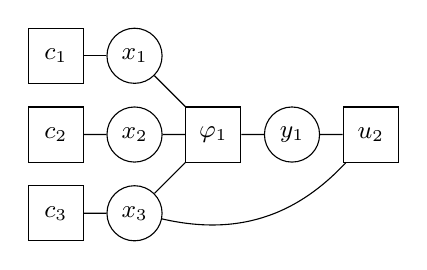
\begin{tikzpicture}[scale=0.8]%,node distance=1.25cm]
        \small
        \tikzstyle{var} = [circle,draw,minimum height=0.7cm]
        \tikzstyle{fac} = [rectangle,draw,minimum width=0.7cm,minimum height=0.7cm]
        \tikzstyle{sen} = [diamond,draw,minimum width=0.7cm,minimum height=0.7cm]
        \node[var] (a1) at (0,0) {$x_1$};
        \node[below of=a1,node distance=0.7cm] (r1) {};
        \node[var,below of=a1] (a2) {$x_2$};
        \node[below of=a2,node distance=0.7cm] (r2) {};
        \node[var,below of=a2] (a3) {$x_3$};
        \node[fac,left of=a1] (u1) {$c_1$};
        \node[fac,left of=a2] (u2) {$c_2$};
        \node[fac,left of=a3] (u3) {$c_3$};
        
        \path (u1) edge (a1);
        \path (u2) edge (a2);
        \path (u3) edge (a3);
        
        \node[fac,right of=a2] (f1) {$\varphi_1$};
        
        \path (a1) edge (f1);
        \path (a2) edge (f1);
        \path (a3) edge (f1);
        
        \node[var,right of=f1] (e1) {$y_1$};
        \node[below of=e1,node distance=1cm] (r3) {};
        
        \path (f1) edge (e1);
        
        \node[fac,right of=e1] (r) {$u_2$};
        
        \path (e1) edge (r);
        \path[bend left] (r) edge (a3);
        
    \end{tikzpicture}

\end{document}